\title{CS 613 - Machine Learning}
\author{
        Assignment 4 - Dimensionality Reduction \\
        Robert Thompson \\
}
\date{}
\documentclass[12pt]{article}
\usepackage[margin=0.7in]{geometry}
\usepackage{graphicx}
\usepackage{float}
\usepackage{comment}
\usepackage{amsmath}
\usepackage{listings}

\includecomment{versionB}
%\excludecomment{versionB}

\begin{document}
\maketitle

\section{Theory Questions}
All of the theory questions will use the following data:
\begin{center}
$X=
 \begin{bmatrix}
	-2 & 1\\
	-5 & -4\\	
	-3 & 1\\
	0 & 3\\
	-8 & 11\\
	-2 & 5\\
	1 & 0\\
	5 & -1\\
	-1 & -3\\
	6 & 1\\
\end{bmatrix},
Y =  \begin{bmatrix}
1\\
1\\
1\\
1\\
1\\
2\\
2\\
2\\
2\\
2\\
\end{bmatrix},
$
\end{center}
\begin{enumerate}
    \item Zscore the data and create a 2D plot of the datapoints, visualizing class one data as squares, and class two data as circles (5pts).
        \begin{enumerate}
            \item Define
        	 $X = 
        	\begin{bmatrix}
        	    -2 & 1\\
                -5 & -4\\	
            	-3 & 1\\
            	0 & 3\\
            	-8 & 11\\
            	-2 & 5\\
            	1 & 0\\
            	5 & -1\\
            	-1 & -3\\
            	6 & 1\\
        	\end{bmatrix}$ \\
            \item Calculate the $X$ Means and Standard Deviations \\ \\
        	$\mu &= \begin{bmatrix} -0.9 & 1.4 \end{bmatrix} $ \\ \\
        	$\sigma &= \begin{bmatrix} 4.23 & 4.27 \end{bmatrix} $ \\ 
	    \item Z-Score our X Data
	    \begin{flalign*}
        X_{zscored}
        &= \begin{bmatrix}
    	    -2 & 1\\
            -5 & -4\\	
        	-3 & 1\\
        	0 & 3\\
        	-8 & 11\\
        	-2 & 5\\
        	1 & 0\\
        	5 & -1\\
        	-1 & -3\\
        	6 & 1
    	\end{bmatrix} - \begin{bmatrix} -0.9 & 1.4 \end{bmatrix} / \begin{bmatrix} 4.23 & 4.27 \end{bmatrix} &\\\\ 
    	&= \begin{bmatrix}
    	   -0.26 & -0.09\\
            -0.97 & -1.26\\	
        	-0.50 & -0.09\\
        	0.21 & 0.37\\
        	-1.68 & 2.25\\
        	-0.26 & 0.84\\
        	0.45 & -0.33\\
        	1.40 & -0.56\\
        	-0.02 & -1.03\\
        	1.63 & -0.09
    	\end{bmatrix}
    	\end{flalign*}
    	\item 2D Class 1 vs. Class 2 Plot
    	\begin{figure}[H]
            \begin{center}
            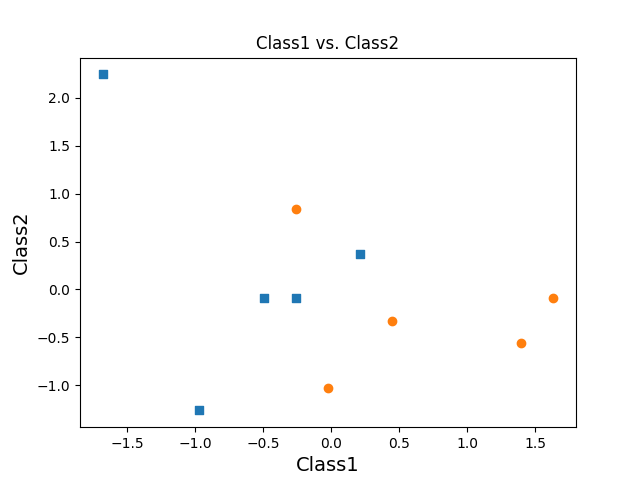
\includegraphics{images/theory_class1_vs._class2.png}
            \label{GD}
            \end{center}
        \end{figure}
        \end{enumerate}
        
    \item PCA
    	\begin{enumerate}
        	\item Find the principle components of the data.  You may use an \emph{eig} function, but show the math leading up to, and after, using that function.  Make sure that your principle components are normalized to be unit length.  (5pts).
        	\begin{enumerate}
        	    \item Transpose our $X_{zscored}$ Data
        	    \begin{flalign*}
                X^T
                &= \begin{bmatrix}
                    -0.26 & -0.97 & -0.50 & 0.21 & -1.68 & -0.26 & 0.45 & 1.40 & -0.02 & 1.63 \\
                    -0.09 & -1.26 & -0.09 & 0.37 & 2.25 & 0.84 & -0.33 & -0.56 & -1.03 & -0.09
            	\end{bmatrix}
            	\end{flalign*}
        	    \item Calculate the Covariance Matrix of our $X_{zscored}$ Data
        	    \begin{flalign*}
                \sum
                &= \frac{X^TX}{N-1} = 
                \begin{bmatrix}
                    -1 & -0.41 \\
                    -0.41 & 1
            	\end{bmatrix}
            	\end{flalign*}
        	    \item Perform Eigendecomposition on the Covariance Matrix \\ \\
        	    Eigenvalues = $\begin{bmatrix} 1.41 & 0.59 \end{bmatrix}$ \\ \\
        	    Eigenvectors = 
        	    $\begin{bmatrix} 
        	        0.71 & 0.71 \\
        	        -0.71 & 0.71
        	    \end{bmatrix}$ \\
        	    \item Determine Largest Eigenvalue and its Associated Eigenvector \\ \\
        	    Largest Eigenvalue = $\begin{bmatrix} 1.41  \end{bmatrix}$ \\ \\
        	    Largest Eigenvectors = 
        	    $\begin{bmatrix} 
        	        0.71 \\
        	        -0.71
        	    \end{bmatrix}$\ \\
        	    \item Project $X_{zscored}$ into Eigenvector Space \\ \\
        	    \begin{flalign*}
                Z = XW
                &= \begin{bmatrix}
                    0.26 & -0.09\\
                    -0.97 & -1.26\\	
                	-0.50 & -0.09\\
                	0.21 & 0.37\\
                	-1.68 & 2.25\\
                	-0.26 & 0.84\\
                	0.45 & -0.33\\
                	1.40 & -0.56\\
                	-0.02 & -1.03\\
                	1.63 & -0.09
            	\end{bmatrix}
            	\begin{bmatrix} 
        	        0.71 \\
        	        -0.71
        	    \end{bmatrix} &\\\\
        	    &= \begin{bmatrix}
                    -0.12\\
                    0.21\\
                    -0.29\\
                    -0.11\\
                    -2.78\\
                    -0.78\\
                    0.55\\
                    1.38\\
                    0.71\\
                    1.22\\
                    \end{bmatrix}
            	\end{flalign*}
        	    
        	\end{enumerate}
            \item Project your data down to 1D using the principle component associated with the largest eigenvalue.  Plot this data in 1D, visualizing class one data as squares, and class two data as circles (3pts).
            \begin{figure}[H]
                \begin{center}
                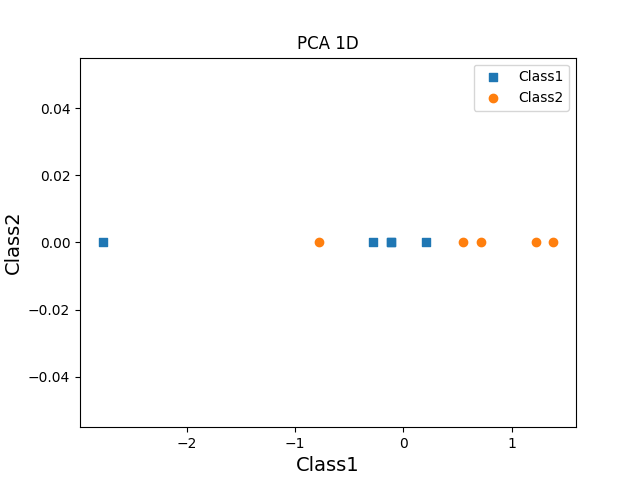
\includegraphics{images/theory_pca_1d.png}
                \label{GD}
                \end{center}
            \end{figure}
        	\item Based on your plot, does the PCA projection provide good class separation?  Why or why not (2pts)? \\
        	Given the 1-dimensional plot of class 1 and class 2 it is extremely easy to see how the classes are separated. There is no overlap between class 1 (squares) and class 2 (circles) on the graph. Therefore, this PCA projection provides a good class separation.
        	
    	\end{enumerate}
    	
    \item LDA
    	\begin{enumerate}
        	\item Using LDA, find the direction of projection (show your work in detail similar to the prior question).  Normalize this vector to be unit length (5pts).
        	\begin{enumerate}
        	    \item Compute the Means for Class 1 and Class 2 \\ \\
        	    $\mu^{(1)} &= \begin{bmatrix} -0.64 & 0.24 \end{bmatrix} $ \\ \\
        	    $\mu^{(2)} &= \begin{bmatrix} 0.64 & -0.24 \end{bmatrix} $ \\
        	    \item Compute Scatter Matrices for Class 1 and Class 2 \\ \\
        	    $\sigma^{(1)^2} &=
        	    \begin{bmatrix}
        	       2.04 & -0.75 \\
        	       -0.75 & 0.27
        	    \end{bmatrix}$ \\ \\
        	    $\sigma^{(2)^2} &=
        	    \begin{bmatrix}
        	       4.08 & -1.50 \\
        	       -1.50 & 0.55
        	    \end{bmatrix}$ \\
        	    \item Compute the Within and Between Class Scatter Matrices \\
        	    \begin{flalign*}
        	    S_{B} = (\mu^{(1)} - \mu^{(2)})^T (\mu^{(1)} - \mu^{(2)}) =
        	    \begin{bmatrix}
                    4.08 & -1.50 \\
                    -1.50 & 0.55
                    \end{bmatrix}
        	    \end{flalign*}
        	    \begin{flalign*}
        	    S_{w} = (\sigma^{(1)^2} + \sigma^{(2)^2}) =
        	    \begin{bmatrix}
                    4.92 & -2.18 \\
                    -2.18 & 8.45
                    \end{bmatrix}
        	    \end{flalign*}
        	    \begin{flalign*}
        	    S_{w}^{-1} = \frac{1}{(4.92*8.45)-(-2.18-(-2.18))}
        	    \begin{bmatrix}
                    8.45 & 2.18 \\
                    2.18 & 4.92
                    \end{bmatrix}
                = \begin{bmatrix}
                    0.23 & 0.06 \\
                    0.06 & 0.13
                    \end{bmatrix}
        	    \end{flalign*}
        	    \item Perform the Eigendecomposition on $S_{W}^{-1}S_{B}$\\ \\
        	    Eigenvalues = $\begin{bmatrix} 8.36\mathrm{e}{-01} & 5.20\mathrm{e}{-18} \end{bmatrix}$ \\ \\
        	    Eigenvectors = 
        	    $\begin{bmatrix} 
        	        0.99 & 0.344 \\
        	        0.05 & 0.94
        	    \end{bmatrix}$ \\
        	    \item Determine Largest Eigenvalue and its Associated Eigenvector \\ \\
        	    Largest Eigenvalue = $\begin{bmatrix} 8.36\mathrm{e}{-01}  \end{bmatrix}$ \\ \\
        	    Largest Eigenvectors = 
        	    $\begin{bmatrix} 
        	        0.99 \\
        	        0.05
        	    \end{bmatrix}$\ \\
        	    \item Project $X_{zscored}$ into Eigenvector Space \\ \\
        	    \begin{flalign*}
                Z = XW
                &= \begin{bmatrix}
                    0.26 & -0.09\\
                    -0.97 & -1.26\\	
                	-0.50 & -0.09\\
                	0.21 & 0.37\\
                	-1.68 & 2.25\\
                	-0.26 & 0.84\\
                	0.45 & -0.33\\
                	1.40 & -0.56\\
                	-0.02 & -1.03\\
                	1.63 & -0.09
            	\end{bmatrix}
            	\begin{bmatrix} 
        	        0.99 \\
        	        0.05
        	    \end{bmatrix} &\\\\
        	    &= \begin{bmatrix}
                    -0.26\\
                    -1.03\\
                    -0.50\\
                    0.23\\
                    -1.57\\
                    -0.22\\
                    0.43\\
                    1.37\\
                    -0.74\\
                    1.63\\
                    \end{bmatrix}
            	\end{flalign*}
        	\end{enumerate}
            \item Project your data down to 1D using the the direction of projection found from the LDA process.  Plot this data in 1D, visualizing class one data as squares and class two data as circles (3pts).
            \begin{figure}[H]
                \begin{center}
                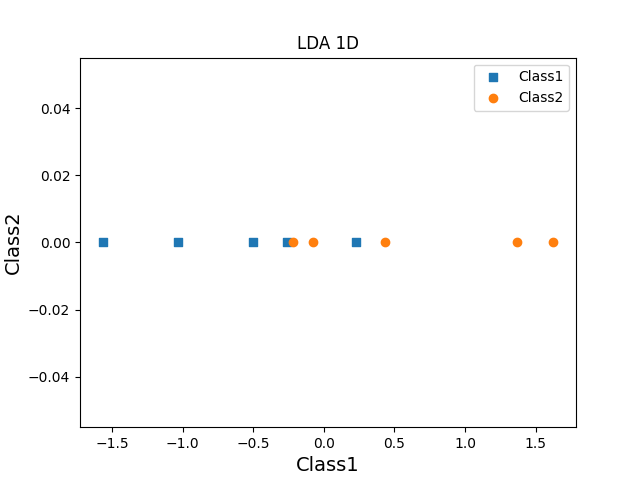
\includegraphics{images/theory_lda_1d.png}
                \label{GD}
                \end{center}
            \end{figure}
        	\item Based on your plot, does the LDA projection provide good class separation?  Why or why not (2pts)? \\
        	Given the 1-dimensional LDA plot of class 1 (squares) and class 2 (circles) it is extremely easy to see how the classes are not fully separated. Therefore, this LDA projection does NOT provide a good class separation.
    	\end{enumerate}
\end{enumerate}


\newpage
\section{Dimensionality Reduction for Visualization}\label{pca}

\begin{enumerate}
    \item Non-Whitened 2D PCA Projected Data
    \begin{figure}[H]
        \begin{center}
        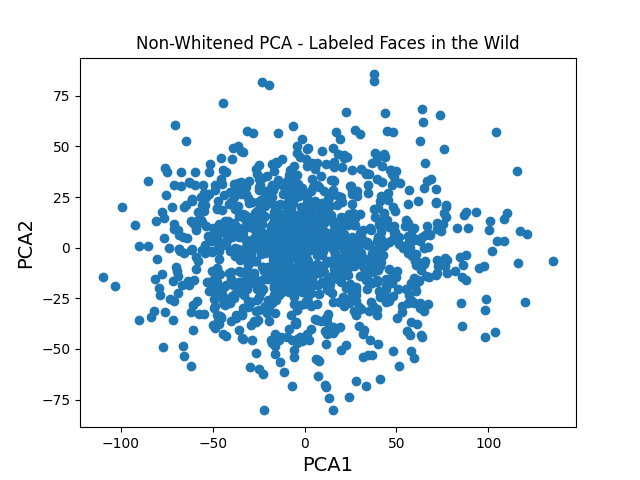
\includegraphics{images/non-whitened_pca.png}
        \label{GD}
        \end{center}
    \end{figure}
    \item Whitened 2D PCA Projected Data
    \begin{figure}[H]
        \begin{center}
        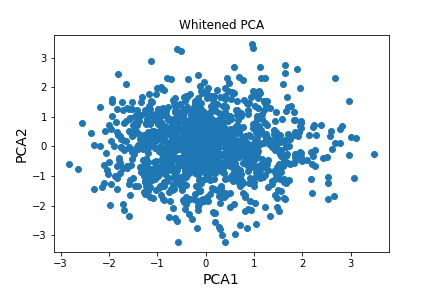
\includegraphics{images/whitened_pca.png}
        \label{GD}
        \end{center}
    \end{figure}
    \item Non-Whitened and Whitened Overlay 2D PCA Projected Data
    \begin{figure}[H]
        \begin{center}
        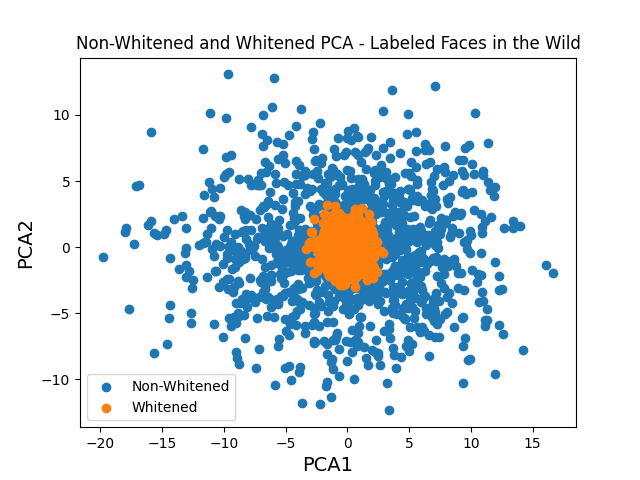
\includegraphics{images/non-whitened_and_whitened_pca.png}
        \label{GD}
        \end{center}
    \end{figure}
\end{enumerate}

\section{Dimensionality Reduction for KNNs}\label{knn}

\begin{enumerate}
    \item Validation Accuracy
    \begin{itemize}
        \item $k=1$ $D=original$: $0.19128329297820823$
        \item $k=1$ $D=100$ PCA: $0.1791767554479419$
        \item $k=1$ $D=100$ PCA Whitened: $0.25181598062953997$
    \end{itemize}
\end{enumerate}

\section{Eigenfaces as Compression}\label{eigenface}

\begin{enumerate}
    \item Primary Component Visualized as an Image
    \begin{figure}[H]
        \begin{center}
        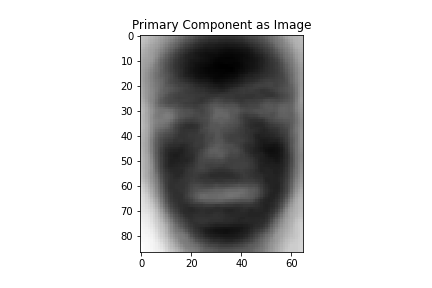
\includegraphics{images/primary_component_as_image.png}
        \label{GD}
        \end{center}
    \end{figure}
    \item Image Used for Compression / Reconstruction
    \begin{figure}[H]
        \begin{center}
        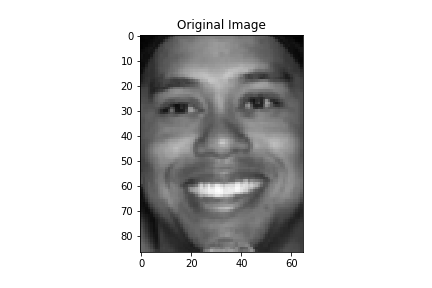
\includegraphics{images/original_image.png}
        \label{GD}
        \end{center}
    \end{figure}
    \item Reconstructed Image Using One Component
    \begin{figure}[H]
        \begin{center}
        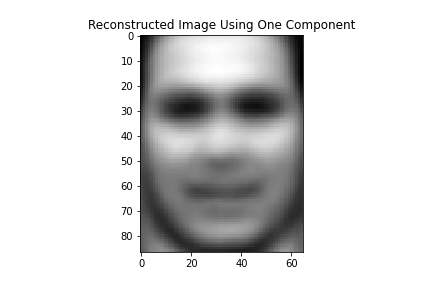
\includegraphics{images/reconstructed_image_using_one_component.png}
        \label{GD}
        \end{center}
    \end{figure}
    \item Minimum Number of Components Necessary to Perform $95\%$ Reconstruction: $181$
    \item Reconstructed Image Using the Minimum Number of Components ($181$)
    \begin{figure}[H]
        \begin{center}
        \includegraphics{images/95_reconstruction_image.png}
        \label{GD}
        \end{center}
    \end{figure}
\end{enumerate}

\end{document}